% Chapter 2: deep neural networks, gene regulation and convolutional neural networks.
% Requires: amsmath, amssymb, bm, graphicx, booktabs, multirow, subcaption,
% tikz (arrows.meta, positioning, calc, decorations.pathreplacing, decorations.pathmorphing, shapes.geometric, fit), natbib.
% Computed figures and the tables figures/pwm_example_table.tex and figures/pwm_scan_table.tex are produced by
% scripts/make_figures.py; figures/slides/ holds figures taken from the lecture slides.

\providecommand{\R}{\mathbb{R}}
\providecommand{\E}{\mathbb{E}}
\providecommand{\Normal}{\mathcal{N}}
\providecommand{\argmax}{\operatorname*{arg\,max}}
\providecommand{\argmin}{\operatorname*{arg\,min}}
\providecommand{\vy}{\mathbf{y}}
\providecommand{\vx}{\mathbf{x}}
\providecommand{\mX}{\mathbf{X}}
\providecommand{\mI}{\mathbf{I}}
\providecommand{\vb}{\boldsymbol{\beta}}
\providecommand{\veps}{\boldsymbol{\epsilon}}
\providecommand{\vp}{\mathbf{p}}
\providecommand{\vg}{\mathbf{g}}
\providecommand{\ind}{\mathbf{1}}
\providecommand{\mB}{\mathbf{B}}
\providecommand{\mA}{\mathbf{A}}
\providecommand{\mW}{\mathbf{W}}
\providecommand{\mP}{\mathbf{P}}
\providecommand{\mY}{\mathbf{Y}}
\providecommand{\mZ}{\mathbf{Z}}
\providecommand{\vh}{\mathbf{h}}
\providecommand{\vo}{\mathbf{o}}
\providecommand{\vu}{\mathbf{u}}
\providecommand{\vc}{\mathbf{c}}
\providecommand{\vm}{\mathbf{m}}
\providecommand{\vv}{\mathbf{v}}
\providecommand{\va}{\boldsymbol{\alpha}}
\providecommand{\vtheta}{\boldsymbol{\theta}}
\providecommand{\vdelta}{\boldsymbol{\delta}}
\providecommand{\Loss}{\mathcal{L}}
\providecommand{\vgamma}{\boldsymbol{\gamma}}

\chapter{Deep neural networks and gene regulation}
\label{ch:cnn}

Chapter 1 developed linear models for predicting a response, such as drug sensitivity, from features, such as gene expression. This chapter has three parts. The first extends those models to deep neural networks, which can represent nonlinear functions and interactions between features, and describes how they are fit: backpropagation to compute gradients and stochastic gradient descent to use them. The second part returns to biology and asks \emph{how} cells control which genes are expressed. A central mechanism is the binding of transcription factors to short DNA sequence patterns called motifs, which can be measured genome-wide with ChIP-seq. The third part brings the two together. The classical model of transcription factor binding, the position weight matrix, turns out to be a single convolutional filter, and stacking such filters with nonlinearities and pooling gives a convolutional neural network (CNN) that predicts binding from DNA sequence.

%======================================================================
\section{Beyond linear models}
\label{sec:beyond_linear}
%======================================================================

Linear models have two limitations that matter in practice (Figure~\ref{fig:limitations}). The first is \emph{nonlinearity}. If the response depends on a feature through a curve, a straight line fits poorly however much data we have. The second, less obvious, limitation is the absence of \emph{interaction effects}. An interaction is present when the effect of one feature on the response depends on the value of another. In the classification example of Figure~\ref{fig:limitations}b the positive samples occupy a bounded region of the $(x_1,x_2)$ plane, and no single line separates them from the negatives.

A classical fix is to add interaction terms to a linear model. With two features,
\begin{equation}
  y_i = \beta_1 x_{i1} + \beta_2 x_{i2} + \beta_{12}x_{i1}x_{i2} + \epsilon_i ,
\end{equation}
where $\beta_{12}\in\R$ is the interaction coefficient, or, for classification, $p(y_i=1\mid\vx_i)=\sigma(\beta_1x_{i1}+\beta_2x_{i2}+\beta_{12}x_{i1}x_{i2})$ with $\sigma$ the logistic function of Chapter 1. Polynomial terms such as $x_{i1}^2$ can similarly capture curvature. This works for a handful of features but does not scale. With $P$ features there are $P(P-1)/2$ pairwise interactions; for $P=20{,}000$ genes that is about $2\times10^8$ coefficients, before considering three-way interactions or curvature. We need models that learn which nonlinear combinations of features matter, rather than enumerating them.

\begin{figure}[t]
  \centering
  \begin{subfigure}[b]{0.48\linewidth}
    \includegraphics[width=\linewidth]{limitations_nonlinear.pdf}
    \caption{}
  \end{subfigure}\hfill
  \begin{subfigure}[b]{0.48\linewidth}
    \includegraphics[width=\linewidth]{limitations_interaction.pdf}
    \caption{}
  \end{subfigure}
  \caption{Two limitations of linear models, on simulated data. (a) Nonlinearity: the least-squares line misses the curved relationship between $x$ and $y$, which a small neural network captures. (b) Interaction: positives ($+$) lie inside a disc and negatives ($-$) outside. The logistic regression decision boundary ($p=0.5$) is a line and cannot enclose the positives; a neural network classifier's boundary can.}
  \label{fig:limitations}
\end{figure}

Many nonlinear methods exist. Kernel methods, including support vector machines and Gaussian processes, implicitly map the features into a high-dimensional space in which a linear model is fit. Decision trees partition the feature space by a sequence of thresholds on single features, and ensembles of trees (random forests and gradient boosting) are among the most accurate methods for tabular data. We focus on neural networks because they are the basis of most current models of genomic sequence, and because they are fit with the same gradient-based machinery as the linear models of Chapter 1.

%======================================================================
\section{Neural networks}
\label{sec:mlp}
%======================================================================

\subsection{From logistic regression to a hidden layer}

Recall logistic regression for sample $i$ with features $\vx_i\in\R^P$: the linear predictor $g_i=\vx_i^\top\vb$ is passed through the logistic sigmoid to give a probability. A neural network keeps this building block but uses many copies of it. Let $H$ be the number of \emph{hidden units} (or neurons). Hidden unit $k\in\{1,\dots,H\}$ has its own coefficient vector $\vb_k\in\R^P$ and computes
\begin{equation}
  h_{ik} = \sigma\big(\underbrace{\vx_i^\top}_{1\times P}\underbrace{\vb_k}_{P\times1}\big),
\end{equation}
where $\sigma:\R\to\R$ is a fixed nonlinear \emph{activation function}. Stacking the columns $\vb_1,\dots,\vb_H$ into a weight matrix $\mB\in\R^{P\times H}$, the whole \emph{hidden layer} is
\begin{equation}
  \underbrace{\vh_i^\top}_{1\times H} = \sigma\big(\underbrace{\vx_i^\top}_{1\times P}\underbrace{\mB}_{P\times H}\big),
  \label{eq:hidden}
\end{equation}
with $\sigma$ applied elementwise. The \emph{output layer} is a linear function of the hidden units. With $D$ outputs and a second weight matrix $\mA\in\R^{H\times D}$ whose $d$-th column is $\va_d\in\R^H$,
\begin{equation}
  o_{id} = \vh_i^\top\va_d, \qquad \underbrace{\vo_i^\top}_{1\times D} = \underbrace{\vh_i^\top}_{1\times H}\underbrace{\mA}_{H\times D}.
  \label{eq:output}
\end{equation}
Intercepts (called \emph{biases} in the neural network literature) are included by appending a constant 1 to $\vx_i$ and to $\vh_i$, as in Chapter 1; we leave them implicit. The network is drawn as a graph in Figure~\ref{fig:mlp}, with one node per input, hidden unit and output, and one edge per weight: the edge from $x_{ip}$ to $h_{ik}$ carries $B_{pk}$.

The outputs $\vo_i\in\R^D$ are used exactly as the linear predictor was in Chapter 1. For regression, $\vo_i$ is the prediction of a continuous response and the loss is the squared error. For binary classification, $D=1$ and $\sigma(o_i)$ is the probability that $y_i=1$, with the binary cross-entropy loss. For multiclass classification, $D$ is the number of classes, the softmax of $\vo_i$ gives a probability vector, and the loss is the cross-entropy. Logistic regression is the special case with no hidden layer.

\begin{figure}[t]
  \centering
  \begin{tikzpicture}[>=Stealth, every node/.style={font=\small},
      unit/.style={circle, draw, minimum size=0.8cm, inner sep=0pt}]
    \foreach \j/\lab in {1/$x_{i1}$, 2/$x_{i2}$, 3/$x_{i3}$}
      \node[unit, draw=red!70!black] (x\j) at ({1.6*\j+0.8}, 0) {\lab};
    \foreach \k/\lab in {1/$h_{i1}$, 2/$h_{i2}$, 3/$h_{i3}$, 4/$h_{i4}$}
      \node[unit, draw=blue!70!black] (h\k) at ({1.6*\k}, -1.8) {\lab};
    \foreach \d/\lab in {1/$o_{i1}$, 2/$o_{i2}$}
      \node[unit, draw=green!50!black] (o\d) at ({1.6*\d+1.6}, -3.6) {\lab};
    \foreach \j in {1,2,3} \foreach \k in {1,2,3,4} \draw[->, gray] (x\j) -- (h\k);
    \foreach \k in {1,2,3,4} \foreach \d in {1,2} \draw[->, gray] (h\k) -- (o\d);
    \draw[->, thick] (x1) -- node[left, pos=0.45] {$B_{12}$} (h2);
    \node[right, align=left] at (7.3,0) {input, $\vx_i\in\R^P$};
    \node[right, align=left] at (7.3,-1.8) {hidden, $\vh_i^\top=\sigma(\vx_i^\top\mB)$, $\mB\in\R^{P\times H}$};
    \node[right, align=left] at (7.3,-3.6) {output, $\vo_i^\top=\vh_i^\top\mA$, $\mA\in\R^{H\times D}$};
  \end{tikzpicture}
  \caption{A neural network with one hidden layer, here with $P=3$ inputs, $H=4$ hidden units and $D=2$ outputs. Each edge carries one weight; the highlighted edge from $x_{i1}$ to $h_{i2}$ carries $B_{12}$.}
  \label{fig:mlp}
\end{figure}

\subsection{Activation functions}

Early neural networks used the logistic sigmoid as the activation function. Most current networks use the \emph{rectified linear unit} (ReLU)~\citep{nair2010},
\begin{equation}
  \operatorname{ReLU}(z) = \max(z,0),
\end{equation}
which is zero for negative inputs and the identity for positive inputs. Smooth variants such as the Gaussian error linear unit, $\operatorname{GELU}(z)=z\,\Phi(z)$ with $\Phi$ the standard normal cumulative distribution function~\citep{hendrycks2016}, are common in large models (Figure~\ref{fig:activations}). The ReLU's gradient is 1 for any positive input, whereas the sigmoid's gradient $\sigma(z)(1-\sigma(z))$ vanishes for large $|z|$, which slows gradient-based training of deep networks.

The nonlinearity is essential. Without it, $\vo_i^\top=\vx_i^\top\mB\mA$, which is a linear model with coefficient matrix $\mB\mA\in\R^{P\times D}$. Adding layers to a linear network adds parameters but not expressive power.

\begin{figure}[t]
  \centering
  \includegraphics[width=\linewidth]{activations.pdf}
  \caption{Common activation functions. $\Phi$ is the standard normal cumulative distribution function.}
  \label{fig:activations}
\end{figure}

\subsection{Deep networks}

Hidden layers can be stacked. Let $\vh_i^{(0)}=\vx_i$ and $H_0=P$. A network with $M$ hidden layers of widths $H_1,\dots,H_M$ computes
\begin{equation}
  \vh_i^{(m)\top} = \sigma\big(\vh_i^{(m-1)\top}\mB^{(m)}\big), \quad m=1,\dots,M, \qquad \vo_i^\top = \vh_i^{(M)\top}\mA,
\end{equation}
with weight matrices $\mB^{(m)}\in\R^{H_{m-1}\times H_m}$ and $\mA\in\R^{H_M\times D}$. This architecture, in which every unit in one layer connects to every unit in the next, is called a \emph{fully connected} or \emph{dense} network, or a \emph{multilayer perceptron} (MLP), a name that dates from early models of neurons. ``Deep'' refers to having more than one hidden layer.

What functions does an MLP represent? With ReLU activations each hidden unit is a linear function of its inputs followed by a hinge, so the network computes a continuous, piecewise linear function of $\vx_i$. Each layer can bend the function in new places, so deeper networks divide the input space into more linear pieces. Figure~\ref{fig:mlp_random} shows functions of a one-dimensional input computed by small MLPs with random weights: with one hidden layer of five units there are at most five kinks, while with four hidden layers the function is considerably more complex. A one-hidden-layer network can approximate any continuous function on a bounded domain arbitrarily well if $H$ is large enough~\citep{hornik1989}, but deeper networks can represent many functions with far fewer units.

\begin{figure}[t]
  \centering
  \includegraphics[width=\linewidth]{mlp_random.pdf}
  \caption{Functions computed by ReLU MLPs with one input, $M$ hidden layers of five units and one output, with weights and biases drawn from $\Normal(0,1)$. Each colour is a different random network; outputs are standardized for display. The functions are continuous and piecewise linear, with more pieces as depth increases.}
  \label{fig:mlp_random}
\end{figure}

A network with thousands or millions of parameters can fit its training data perfectly, so overfitting is a real risk. Deep learning practice combines very flexible models with regularization: L2 penalties on the weights (called weight decay), early stopping based on validation loss, dropout, data augmentation and others. Even so, large networks often generalize better than classical theory based on parameter counts would predict~\citep{zhang2017}. One explanation is that gradient-based training tends to find minima of the loss that occupy a large volume of parameter space (``flat'' minima), and these tend to generalize well~\citep{hochreiter1997}. Why this works so well is still an active research question. In practice, repeated training runs from different random initializations usually reach similar performance, although the fitted weights differ.

%======================================================================
\section{Backpropagation}
\label{sec:backprop}
%======================================================================

To fit a neural network by gradient descent we need the gradient of the loss with respect to every weight. Chapter 1 computed the logistic regression gradient by the chain rule along a computational graph. Neural networks are deeper graphs, and the same idea, applied systematically, is \emph{backpropagation}~\citep{rumelhart1986}.

\subsection{The multivariate chain rule}

For scalars, if $y$ depends on $x$ through $u$, $x\to u\to y$, then $\frac{\partial y}{\partial x}=\frac{\partial y}{\partial u}\frac{\partial u}{\partial x}$. Now let $\vx\in\R^{I}$, $\vu\in\R^{J}$ and $\vy\in\R^{K}$, with $\vu$ a function of $\vx$ and $\vy$ a function of $\vu$. A change in $x_i$ affects $y_k$ through every $u_j$, and the contributions add,
\begin{equation}
  \frac{\partial y_k}{\partial x_i} = \sum_{j=1}^{J}\frac{\partial u_j}{\partial x_i}\frac{\partial y_k}{\partial u_j}.
\end{equation}
Define the gradient matrix $\nabla_{\vx}\vy\in\R^{I\times K}$ by $(\nabla_{\vx}\vy)_{ik}=\partial y_k/\partial x_i$, with one row per input and one column per output, and similarly $\nabla_{\vx}\vu\in\R^{I\times J}$ and $\nabla_{\vu}\vy\in\R^{J\times K}$. The sum is then a matrix product, $(\mathbf{A}\mathbf{C})_{ik}=\sum_j A_{ij}C_{jk}$, so
\begin{equation}
  \underbrace{\nabla_{\vx}\vy}_{I\times K} = \underbrace{(\nabla_{\vx}\vu)}_{I\times J}\,\underbrace{(\nabla_{\vu}\vy)}_{J\times K}.
\end{equation}
For a scalar loss $\ell$, $\nabla_{\vx}\ell\in\R^{I}$ is the usual gradient vector, consistent with Chapter 1. For a longer chain $\vx\to\vu^{(1)}\to\cdots\to\vu^{(M)}\to\ell$, the gradient is a product of $M+1$ matrices. Multiplying from the right, starting at the loss, means every intermediate product is a vector rather than a matrix, which is much cheaper. That is the order backpropagation uses.

\subsection{Gradients of a one-hidden-layer network}

Consider one sample with input $\vx\in\R^P$ and continuous targets $\vy\in\R^D$, a network with sigmoid hidden units, and the squared-error loss. We drop the sample index $i$. The forward pass computes, in order,
\begin{equation}
  \underbrace{\vg^\top}_{1\times H} = \vx^\top\mB, \qquad \vh = \sigma(\vg), \qquad \underbrace{\vo^\top}_{1\times D} = \vh^\top\mA, \qquad \ell = \frac12\sum_{d=1}^D(o_d-y_d)^2,
\end{equation}
where $g_k=\sum_p x_pB_{pk}$ and $o_d=\sum_k h_kA_{kd}$ (Figure~\ref{fig:backprop}). The backward pass applies the chain rule from the loss downward, reusing each derivative once it has been computed.
\begin{enumerate}
  \item Output: $\dfrac{\partial\ell}{\partial o_d} = o_d - y_d$. Write $\vdelta_{o}=\vo-\vy\in\R^D$.
  \item Output weights: $A_{kd}$ affects $\ell$ only through $o_d$, and $\partial o_d/\partial A_{kd}=h_k$, so
  \begin{equation}
    \frac{\partial\ell}{\partial A_{kd}} = \frac{\partial\ell}{\partial o_d}\frac{\partial o_d}{\partial A_{kd}} = (o_d-y_d)\,h_k, \qquad \underbrace{\nabla_{\mA}\ell}_{H\times D} = \underbrace{\vh}_{H\times1}\underbrace{\vdelta_o^\top}_{1\times D}.
  \end{equation}
  \item Hidden units: $h_k$ affects every output, with $\partial o_d/\partial h_k=A_{kd}$, so
  \begin{equation}
    \frac{\partial\ell}{\partial h_k} = \sum_{d=1}^D\frac{\partial\ell}{\partial o_d}\frac{\partial o_d}{\partial h_k} = \sum_{d=1}^D(o_d-y_d)A_{kd}, \qquad \vdelta_h = \mA\vdelta_o\in\R^H.
  \end{equation}
  \item Pre-activations: $h_k=\sigma(g_k)$ and $\sigma'(g)=\sigma(g)(1-\sigma(g))$, so
  \begin{equation}
    \frac{\partial\ell}{\partial g_k} = \frac{\partial\ell}{\partial h_k}\,\sigma'(g_k) = \frac{\partial\ell}{\partial h_k}\,h_k(1-h_k), \qquad \vdelta_g = \vdelta_h\odot\vh\odot(\mathbf{1}-\vh),
  \end{equation}
  where $\odot$ is the elementwise product.
  \item First-layer weights: $B_{pk}$ affects $\ell$ only through $g_k$, and $\partial g_k/\partial B_{pk}=x_p$, so
  \begin{equation}
    \frac{\partial\ell}{\partial B_{pk}} = \frac{\partial\ell}{\partial g_k}\,x_p, \qquad \underbrace{\nabla_{\mB}\ell}_{P\times H} = \underbrace{\vx}_{P\times1}\underbrace{\vdelta_g^\top}_{1\times H}.
  \end{equation}
\end{enumerate}
The pattern generalizes to any depth. The gradient with respect to a weight matrix is the outer product of the layer's input and the ``error signal'' $\vdelta$ arriving from above, and the error signal is passed down a layer by multiplying by the transposed weights and the derivative of the activation. With a ReLU activation, step 4 becomes $\delta_{g,k}=\delta_{h,k}\ind[g_k>0]$. The cost of the backward pass is about the same as that of the forward pass. Libraries such as PyTorch, TensorFlow and JAX build the computational graph during the forward pass and compute these gradients automatically (\emph{automatic differentiation}), so in practice we write only the forward pass.

\begin{figure}[t]
  \centering
  \begin{tikzpicture}[>=Stealth, every node/.style={font=\small}, node distance=0.9cm]
    \node (x) {$\vx\ [P]$};
    \node[right=1.4cm of x] (B) {$\mB\ [P\times H]$};
    \node[below=of $(x)!0.5!(B)$] (g) {$\vg^\top=\vx^\top\mB\ [1\times H]$};
    \node[below=of g] (h) {$\vh=\sigma(\vg)\ [H]$};
    \node[right=1.6cm of h] (A) {$\mA\ [H\times D]$};
    \node[below=of $(h)!0.5!(A)$] (o) {$\vo^\top=\vh^\top\mA\ [1\times D]$};
    \node[below=of o] (l) {$\ell=\frac12\sum_d(o_d-y_d)^2$};
    \draw[->] (x) -- (g); \draw[->] (B) -- (g); \draw[->] (g) -- (h);
    \draw[->] (h) -- (o); \draw[->] (A) -- (o); \draw[->] (o) -- (l);
    \begin{scope}[red!70!black, every node/.style={font=\footnotesize, red!70!black}]
      \node[right=0.3cm of l, align=left] {$\partial\ell/\partial o_d=o_d-y_d$};
      \node[right=0.2cm of o.east, align=left] {$\partial\ell/\partial A_{kd}=(o_d-y_d)h_k$};
      \node[left=0.2cm of h.west, align=right] {$\partial\ell/\partial h_k=\sum_d(o_d-y_d)A_{kd}$};
      \node[left=0.2cm of g.west, align=right] {$\partial\ell/\partial g_k=\frac{\partial\ell}{\partial h_k}\sigma'(g_k)$\\$\partial\ell/\partial B_{pk}=\frac{\partial\ell}{\partial g_k}x_p$};
    \end{scope}
  \end{tikzpicture}
  \caption{Computational graph of a one-hidden-layer network with squared-error loss, with the dimension of each quantity in brackets. The forward pass runs top to bottom; the backward pass (red) computes the derivatives from the bottom up, each from the one below it.}
  \label{fig:backprop}
\end{figure}

%======================================================================
\section{Stochastic gradient descent}
\label{sec:sgd}
%======================================================================

\subsection{Minibatch gradients}

Let $\vtheta$ collect all the weights of the network. The loss over a training set of $N$ samples is usually written as an average,
\begin{equation}
  \Loss(\vtheta) = \frac1N\sum_{i=1}^N\ell_i(\vtheta), \qquad \ell_i(\vtheta)=\ell(\vx_i,\vy_i,\vtheta),
\end{equation}
where $\ell$ is the per-sample loss (squared error, binary cross-entropy or cross-entropy). Averaging rather than summing makes the scale of the loss, and so a good step size, independent of $N$. Gradient descent (Chapter 1) needs $\nabla_{\vtheta}\Loss$, which costs a pass over all $N$ samples per step. Genomic data sets for neural networks often have millions of training sequences, so this is slow.

\emph{Stochastic gradient descent} (SGD) replaces the full gradient by an estimate from a random subset of samples, a \emph{minibatch} $\mathcal{B}\subset\{1,\dots,N\}$ of size $|\mathcal{B}|$,
\begin{equation}
  \nabla_{\vtheta}\Loss_{\mathcal{B}} = \frac{1}{|\mathcal{B}|}\sum_{i\in\mathcal{B}}\nabla_{\vtheta}\ell_i .
\end{equation}
If $\mathcal{B}$ is drawn uniformly at random, each sample $i$ is included with probability $|\mathcal{B}|/N$, so
\begin{equation}
  \E_{\mathcal{B}}\left[\nabla_{\vtheta}\Loss_{\mathcal{B}}\right] = \frac{1}{|\mathcal{B}|}\sum_{i=1}^N\Pr(i\in\mathcal{B})\,\nabla_{\vtheta}\ell_i = \frac{1}{|\mathcal{B}|}\frac{|\mathcal{B}|}{N}\sum_{i=1}^N\nabla_{\vtheta}\ell_i = \nabla_{\vtheta}\Loss .
\end{equation}
The minibatch gradient is an unbiased estimate of the full gradient. The update at iteration $t$ is
\begin{equation}
  \vtheta_{t+1} = \vtheta_t - \alpha_t\nabla_{\vtheta}\Loss_{\mathcal{B}_t}(\vtheta_t),
\end{equation}
with a fresh minibatch $\mathcal{B}_t$ at every step. In practice the training set is shuffled and split into consecutive minibatches; one pass through all of them is an \emph{epoch}.

Because the gradient is noisy, a fixed step size makes the iterates keep bouncing around the minimum. Convergence requires a decreasing step size, with $\sum_t\alpha_t=\infty$ (so the iterates can travel any distance) and $\sum_t\alpha_t^2<\infty$ (so the accumulated noise is finite)~\citep{robbins1951}. The schedule $\alpha_t=c/t$ for a constant $c>0$ satisfies both. Batch size and step size interact: a larger batch reduces the variance of the gradient estimate, roughly in proportion to $1/|\mathcal{B}|$, while a larger step size amplifies the noise. Some noise is not harmful, and is thought to help find minima that generalize well.

\subsection{Adaptive step sizes: Adam}

Choosing a step-size schedule by hand is tedious, and a single scalar $\alpha_t$ treats all parameters alike even though gradients for different weights can differ by orders of magnitude. The most widely used remedy is Adam~\citep{kingma2015}. Let $\vgamma_t=\nabla_{\vtheta}\Loss_{\mathcal{B}_t}(\vtheta_t)$ be the minibatch gradient. Adam keeps exponential moving averages of the gradient and of its elementwise square,
\begin{equation}
  \vm_t = \beta_1\vm_{t-1} + (1-\beta_1)\vgamma_t, \qquad \vv_t = \beta_2\vv_{t-1} + (1-\beta_2)\vgamma_t\odot\vgamma_t,
\end{equation}
starting from $\vm_0=\vv_0=\mathbf{0}$, with decay rates $\beta_1=0.9$ and $\beta_2=0.999$ by default (these $\beta$s are unrelated to regression coefficients). Because the averages start at zero they are biased toward zero early on, which is corrected by $\hat\vm_t=\vm_t/(1-\beta_1^t)$ and $\hat\vv_t=\vv_t/(1-\beta_2^t)$. The update, applied elementwise, is
\begin{equation}
  \vtheta_{t+1} = \vtheta_t - \alpha\frac{\hat\vm_t}{\sqrt{\hat\vv_t}+\varepsilon},
\end{equation}
with a small $\varepsilon$, such as $10^{-8}$, to avoid division by zero. $\hat\vm_t$ estimates the mean gradient and $\hat\vv_t$ its uncentred second moment, so the step in each coordinate is roughly the mean gradient divided by its typical magnitude. In a coordinate where the gradient is large and noisy the step is damped, and in one where it is small but consistent the step is enlarged. Adam can be viewed as a diagonal, noise-aware analogue of the quasi-Newton methods of Chapter 1, which rescale the gradient by an estimate of the curvature. Figure~\ref{fig:sgd} compares full-batch gradient descent, SGD and Adam on a logistic regression loss.

\begin{figure}[t]
  \centering
  \includegraphics[width=\linewidth]{sgd_paths.pdf}
  \caption{150 iterations of three optimizers on the logistic regression loss for simulated data ($N=1000$, two features, no intercept), starting from the black dot; grey lines are loss contours and the cross marks the minimum. Gradient descent uses all $N$ samples per step and follows a smooth path. SGD and Adam use minibatches of 10 samples, so each step costs 1\% as much but the paths are noisy.}
  \label{fig:sgd}
\end{figure}

%======================================================================
\section{Gene regulation}
\label{sec:generegulation}
%======================================================================

Chapter 1 defined a gene's expression as the number of RNA copies of the gene in a cell, and gene regulation as the control of \emph{when} (for example at different stages of development), \emph{where} (in which tissues and cell types) and \emph{why} (in response to which stimuli) a gene is expressed. We now turn to \emph{how} cells achieve this. There are several reasons to care.
\begin{itemize}
  \item \emph{Basic biology}. Every cell in the body has essentially the same genome, yet a neuron, a liver cell and a muscle cell behave very differently. Much of the difference comes from which genes are expressed, and so from how the same DNA sequence is read out differently in each cell type.
  \item \emph{Understanding disease}. Most genetic variants associated with disease risk lie outside protein-coding sequence and are thought to act by changing gene regulation. Cancers and other diseases often involve regulatory programs that have gone wrong.
  \item \emph{Bioengineering}. Gene therapies are safer if the therapeutic gene is active only in the target cell type, which requires designing regulatory DNA sequence with the desired activity.
\end{itemize}

\subsection{Transcription and transcription factors}

Transcription is the synthesis of an RNA copy of a gene from its DNA template (Figure~\ref{fig:transcription}). A gene starts at the \emph{transcription start site} (TSS) and ends at the \emph{transcription end site} (TES). The enzyme that transcribes protein-coding genes is RNA polymerase II (Pol II). Pol II is recruited to the DNA near the TSS (initiation), separates the two strands and moves along the template strand, synthesizing RNA from its $5'$ end (elongation), until it stops and releases the RNA (termination). Pol II needs the help of many other proteins.

Of these, the \emph{transcription factors} (TFs) are the most important for regulation. A TF is a protein with a DNA-binding domain that gives it an affinity for particular short DNA sequences. Humans have about 1,600 TFs~\citep{lambert2018}. Activating TFs bind near a gene and help recruit Pol II, increasing transcription; repressive TFs block Pol II or other TFs, decreasing it. Binding is dynamic: a TF binds, falls off and rebinds, and many TFs with different preferences compete for access to the DNA, so binding at any one site is stochastic. A TF typically regulates hundreds of genes, which lets a cell switch whole programs on together. For example, during an immune response, TFs activated by the infection signal upregulate the genes needed to fight it.

The sequences that a TF prefers are called its \emph{motif}. A motif is a short pattern, typically 6--20 base pairs (bp), such as GATA for the GATA family of TFs. TF binding sites are found in the promoter, the region immediately upstream of the TSS, and in \emph{enhancers}, regulatory regions that can be thousands of base pairs from the gene they regulate. Chapter 3 discusses enhancers and chromatin in more detail.

\begin{figure}[t]
  \centering
  \begin{tikzpicture}[>=Stealth, every node/.style={font=\small}]
    \draw[thick] (0,0.08) .. controls (4,0.08) and (7,0.3) .. (8.2,1.2) .. controls (9,1.8) .. (10.5,2.0);
    \draw[thick] (0,-0.08) .. controls (4,-0.08) and (5.4,-0.1) .. (6.6,-0.35) .. controls (8.4,-0.7) and (9.6,0.9) .. (10.6,1.8);
    \node[left] at (0,0) {DNA};
    \draw[green!50!black, thick] (1.3,0.05) circle (0.48); \node[green!50!black, align=center] at (1.3,1.0) {repressive\\TF};
    \draw[red!70!black, thick] (2.6,0.05) circle (0.48); \node[red!70!black, align=center] at (2.6,-0.95) {activating\\TF};
    \draw[blue!70!black, thick] (4.3,0.05) circle (0.48); \node[blue!70!black] at (4.3,0.85) {Pol II};
    \draw[->, red!70!black, thick] (3.1,0.05) -- (3.8,0.05);
    \draw[-|, green!50!black, thick] (1.5,0.53) to[out=40, in=140] (4.1,0.6);
    \draw[->] (3.5,1.55) node[above] {TSS} -- (3.5,0.15);
    \draw[orange!80!black, thick] (4.0,0.0) .. controls (5.0,0.0) and (5.6,0.4) .. (6.0,1.6) node[above] {RNA};
    \draw[thick] (9.7,1.4) -- (9.9,2.2);
    \draw[->] (10.4,0.5) node[below, align=center] {TES} -- (9.9,1.35);
  \end{tikzpicture}
  \caption{Transcriptional regulation. RNA polymerase II (Pol II) binds near the transcription start site (TSS), separates the DNA strands and synthesizes RNA until the transcription end site (TES). Activating transcription factors bound nearby recruit Pol II; repressive transcription factors block it.}
  \label{fig:transcription}
\end{figure}

%======================================================================
\section{Measuring transcription factor binding with ChIP-seq}
\label{sec:chipseq}
%======================================================================

\subsection{The assay}

Chromatin immunoprecipitation followed by sequencing (ChIP-seq)~\citep{johnson2007,park2009} measures where in the genome a chosen protein is bound. \emph{Chromatin} is DNA together with the proteins bound to it. Like RNA-seq in Chapter 1, ChIP-seq converts the quantity of interest into DNA fragments that can be sequenced (Figure~\ref{fig:chipseq_protocol}).
\begin{enumerate}
  \item \emph{Cross-linking}. Cells are treated, typically with formaldehyde, to form covalent bonds between proteins and the DNA they are touching, so that transiently bound TFs are fixed in place.
  \item \emph{Fragmentation}. The chromatin is broken into fragments of a few hundred base pairs, by sonication or enzymatic digestion.
  \item \emph{Immunoprecipitation} (IP). An antibody that recognizes the TF of interest is used to pull down the TF together with the DNA fragments cross-linked to it. Antibodies are proteins made by the immune system that bind a specific target; antibodies against many TFs are available commercially.
  \item \emph{Purification}. The cross-links are reversed and the proteins, including the antibody and TF, are digested with a protease, leaving the DNA fragments that were bound.
  \item \emph{Sequencing and alignment}. The fragments are sequenced, and the reads are aligned to the genome.
\end{enumerate}
Reads pile up where the TF was bound. One limitation is that each experiment measures one TF, with one antibody, in one cell type or condition.

\begin{figure}[t]
  \centering
  \begin{tikzpicture}[>=Stealth, every node/.style={font=\small, align=center}]
    % chromatin with TFs and antibodies
    \draw[thick] (0,0) .. controls (0.8,0.4) and (1.4,-0.3) .. (2.2,0.2) .. controls (2.8,0.6) and (3.2,0.3) .. (3.6,0.5);
    \draw[red!70!black, thick] (0.9,0.12) circle (0.18); \draw[red!70!black, thick] (2.9,0.45) circle (0.18);
    \foreach \x/\y in {0.9/0.12, 2.9/0.45} {
      \draw[green!50!black, thick] (\x,\y-0.2) -- (\x,\y-0.55); \draw[green!50!black, thick] (\x,\y-0.55) -- (\x-0.15,\y-0.75); \draw[green!50!black, thick] (\x,\y-0.55) -- (\x+0.15,\y-0.75);}
    \node[red!70!black] at (1.9,0.95) {TF};
    \node[green!50!black] at (1.9,-0.9) {antibody};
    \node at (1.8,-1.6) {cross-link,\\fragment};
    \draw[->, thick] (4.0,0.2) -- node[above] {IP} (5.2,0.2);
    % pulled-down fragments
    \foreach \x in {5.7, 6.9} {
      \draw[thick] (\x-0.35,0.25) -- (\x+0.35,0.15);
      \draw[red!70!black, thick] (\x,0.2) circle (0.16);
      \draw[green!50!black, thick] (\x,0.03) -- (\x,-0.3); \draw[green!50!black, thick] (\x,-0.3) -- (\x-0.13,-0.48); \draw[green!50!black, thick] (\x,-0.3) -- (\x+0.13,-0.48);}
    \draw[->, thick] (7.6,0.2) -- node[above] {remove} node[below] {protein} (8.9,0.2);
    \foreach \x in {9.3, 10.1} \draw[thick] (\x,0.25) -- (\x+0.6,0.15);
    \draw[->, thick] (9.9,-0.2) -- node[right] {sequence} (9.9,-1.2);
    \node at (9.9,-1.55) {reads};
    \draw[->, thick] (9.3,-1.55) -- node[above] {align to genome} (6.3,-1.55);
    % coverage
    \begin{scope}[shift={(3.0,-2.6)}]
      \draw (0,0) -- (3.2,0);
      \foreach \h [count=\k] in {0.05,0.08,0.06,0.15,0.4,0.8,0.95,0.7,0.35,0.12,0.06,0.05,0.07,0.04,0.05}
        \fill[red!60] ({0.2*\k-0.15},0) rectangle ({0.2*\k+0.03},\h);
      \node[below] at (1.6,0) {genome position};
    \end{scope}
    \node at (8.0,-2.4) {peak: where the\\TF was bound};
  \end{tikzpicture}
  \caption{ChIP-seq. Proteins are cross-linked to DNA, chromatin is fragmented, and an antibody against the transcription factor (TF) pulls down the TF with its bound DNA. After the protein is removed, the DNA is sequenced and the reads are aligned. Read coverage forms a peak where the TF was bound.}
  \label{fig:chipseq_protocol}
\end{figure}

\subsection{Peaks}

Figure~\ref{fig:igb} shows ChIP-seq data at three zoom levels. Across a whole chromosome (a), many binding sites are detected. Around a single gene (b), the read coverage is low and noisy almost everywhere, with sharp peaks at a few locations, including the TSS. At the finest scale (c), a peak spans a few hundred base pairs, the length of the sequenced fragments, and a sequence match to the TF's motif lies near its summit.

\begin{figure}[t]
  \centering
  \includegraphics[width=0.85\linewidth]{slides/chipseq_igb.jpg}
  \caption{ChIP-seq data viewed in a genome browser. (a) Peaks called by MACS (top track) and genes (RefGene) along a whole chromosome. (b) Read coverage (ChIP-seq WIG track) around the gene \textit{Hs6st1}; peaks are called at the TSS and at several other sites, with grey marking lower-confidence peaks. (c) Zoom on two peaks, each a few hundred base pairs wide, with the TF's motif near the summit. Reproduced from \citet{freese2016}.}
  \label{fig:igb}
\end{figure}

\emph{Peak calling} decides where coverage is higher than expected by chance. Algorithms such as MACS~\citep{zhang2008} slide a window of width comparable to the fragment length along the genome and model the number of reads $Y$ falling in the window. Under the null hypothesis of no binding, reads land at random, so $Y\sim\text{Poisson}(\lambda)$, where $\lambda$ is the expected number of background reads in the window. The p-value for observing $y$ reads is
\begin{equation}
  \Pr(Y\geq y) = 1-\sum_{k=0}^{y-1}\frac{e^{-\lambda}\lambda^k}{k!}.
\end{equation}
For example, with $\lambda=2$, observing 15 or more reads has probability $3.9\times10^{-9}$, while with $\lambda=5$ it has probability $2.3\times10^{-4}$. Since the human genome contains about $10^7$ non-overlapping windows of 300\,bp, only the first is convincing after correcting for multiple testing. The background rate is not uniform along the genome, because some regions are easier to fragment or sequence, so MACS estimates $\lambda$ locally, using a control experiment without immunoprecipitation (``input'') where available. The output is a set of peaks, genomic intervals where the TF is inferred to bind, each with a significance score.

%======================================================================
\section{Motifs and regulatory grammar}
\label{sec:grammar}
%======================================================================

To a first approximation, a TF binds where its motif occurs. Reality is more complicated, because motifs combine~\citep{spitz2012} (Figure~\ref{fig:grammar}).
\begin{itemize}
  \item \emph{Homotypic clusters}. Regulatory sequences often contain several copies of the same motif, which together give stronger or more reliable binding than one copy.
  \item \emph{Heterotypic clusters}. Regulatory sequences are often bound by combinations of different TFs. TFs that bind next to each other can also bind each other, which stabilizes both. A well-studied example is the pair SOX2 and OCT4, which bind adjacent motifs in the regulatory regions of genes that maintain pluripotency in embryonic stem cells (Figure~\ref{fig:sox2oct4}).
  \item \emph{Spatial grammar}. For some combinations, binding or activity depends on the spacing, order and orientation of the motifs.
\end{itemize}
By analogy with language, motifs are words, and the rules by which they combine are a \emph{grammar}. Predicting where a TF binds therefore requires more than finding its motif: it requires a model of how motifs combine.

\begin{figure}[t]
  \centering
  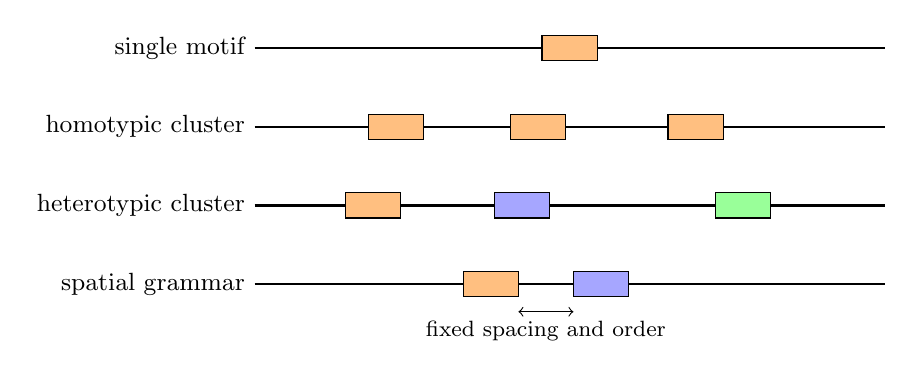
\begin{tikzpicture}[every node/.style={font=\small}, motif/.style={draw, minimum width=0.7cm, minimum height=0.32cm, inner sep=0pt}]
    \foreach \row/\lab in {0/single motif, 1/homotypic cluster, 2/heterotypic cluster, 3/spatial grammar}
      { \draw[thick] (0,-\row) -- (8,-\row); \node[left] at (0,-\row) {\lab}; }
    \node[motif, fill=orange!50] at (4,0) {};
    \foreach \x in {1.8,3.6,5.6} \node[motif, fill=orange!50] at (\x,-1) {};
    \node[motif, fill=orange!50] at (1.5,-2) {}; \node[motif, fill=blue!35] at (3.4,-2) {}; \node[motif, fill=green!40] at (6.2,-2) {};
    \node[motif, fill=orange!50] at (3.0,-3) {}; \node[motif, fill=blue!35] at (4.4,-3) {};
    \draw[<->] (3.35,-3.35) -- node[below, font=\footnotesize] {fixed spacing and order} (4.05,-3.35);
  \end{tikzpicture}
  \caption{Arrangements of transcription factor motifs (boxes; colours denote different TFs) in regulatory DNA. Homotypic clusters repeat one motif; heterotypic clusters combine motifs of different TFs; in a spatial grammar the spacing, order or orientation of the motifs matters.}
  \label{fig:grammar}
\end{figure}

\begin{figure}[t]
  \centering
  \includegraphics[width=0.4\linewidth]{slides/sox2_oct4_motifs.jpg}
  \caption{A heterotypic motif pair. (A) Adjacent SOX2 (HMG domain) and OCT4 (POU domain) binding sites in regulatory regions of five genes expressed in pluripotent stem cells. (B) Sequence logos of the motifs enriched in OCT4 and SOX2 ChIP-seq peaks, which both show the composite motif. Reproduced from \citet{rizzino2016}.}
  \label{fig:sox2oct4}
\end{figure}

\subsection{Sequence-to-function models}

ChIP-seq provides training data for a supervised learning problem (Figure~\ref{fig:seq2fun}). Take a set of DNA sequences of fixed length, for example 200--1000\,bp centred on ChIP-seq peaks (label $y=1$, bound) and an equal number from elsewhere in the genome (label $y=0$, unbound). The task is to learn a function $F$ from a sequence $S$ to the probability that the TF binds it. There are two motivations.
\begin{enumerate}
  \item \emph{Understanding}: what sequence features determine binding, and how do TFs cooperate?
  \item \emph{Prediction of variant effects}: if a mutation in a tumour or a genetic variant associated with a disease changes a regulatory sequence, does it change binding? Applying $F$ to the reference and the altered sequence answers this without a new experiment.
\end{enumerate}
The rest of this chapter develops two choices of $F$: the classical position weight matrix and the convolutional neural network.

\begin{figure}[t]
  \centering
  \begin{tikzpicture}[>=Stealth, every node/.style={font=\small}]
    \foreach \s/\y/\l in {ACGGATAAGTC/0.9/1, TTGATAACCGA/0.45/1, CAGATAAGGTT/0/1, GTCCATTGCAA/-0.6/0, ACCTGTGCATG/-1.05/0, TTACGGCGTAC/-1.5/0}
      { \node[font=\ttfamily\small] at (0,\y) {\s}; \node at (6.2,\y) {$y=\l$}; \draw[->] (1.3,\y) -- (2.3,-0.3); \draw[->] (3.9,-0.3) -- (5.6,\y); }
    \node[draw, rounded corners, minimum width=1.6cm, minimum height=0.9cm, align=center] at (3.1,-0.3) {classifier\\$F(S)$};
    \node at (0,1.45) {DNA sequences $S$};
    \node[align=center] at (7.4,0.45) {bound};
    \node[align=center] at (7.4,-1.05) {unbound};
  \end{tikzpicture}
  \caption{Predicting transcription factor binding as binary classification. Sequences under ChIP-seq peaks are labelled bound and sequences elsewhere unbound; a classifier $F$ maps sequence to the probability of binding.}
  \label{fig:seq2fun}
\end{figure}

%======================================================================
\section{Position weight matrices}
\label{sec:pwm}
%======================================================================

Before neural networks, TF binding was modelled with \emph{position weight matrices} (PWMs)~\citep{stormo2000}. A PWM is a simple probabilistic model that will turn out to be the first layer of a CNN.

\subsection{A probabilistic model of bound sequences}

Consider sequences of a fixed length $K$, typically between 6 and 20. Write a sequence as $x=(x_1,\dots,x_K)$ with $x_k\in\{\mathrm{A},\mathrm{C},\mathrm{G},\mathrm{T}\}$, and let $b\in\{0,1\}$ indicate whether the TF binds it ($b=1$) or not ($b=0$). We build two models for the sequence, one for bound and one for unbound sequences, and combine them with Bayes' rule.

For bound sequences, assume that the nucleotides at different positions are independent, but not identically distributed: each position $k$ has its own distribution over the four nucleotides. Let $\mP\in[0,1]^{4\times K}$ be the \emph{position probability matrix}, with rows indexed by nucleotide $n$ and columns by position $k$,
\begin{equation}
  P_{n,k} = \Pr(x_k=n\mid b=1), \qquad \sum_{n}P_{n,k}=1 .
\end{equation}
Each column of $\mP$ is a probability vector. By independence across positions,
\begin{equation}
  \Pr(x\mid b=1) = \prod_{k=1}^K\Pr(x_k\mid b=1) = \prod_{k=1}^K P_{x_k,k},
\end{equation}
where $P_{x_k,k}$ is the entry in the row of the nucleotide actually present at position $k$ and the column of position $k$. For unbound sequences we use a \emph{background} model in which every position has the same distribution $q_n$, usually the uniform $q_n=\frac14$ (or the genome-wide nucleotide frequencies),
\begin{equation}
  \Pr(x\mid b=0) = \prod_{k=1}^K q_{x_k} = \left(\tfrac14\right)^K .
\end{equation}

Let $\pi=\Pr(b=1)$ be the prior probability of binding. By Bayes' rule and the law of total probability, $\Pr(x)=\Pr(x\mid b=1)\pi+\Pr(x\mid b=0)(1-\pi)$, so
\begin{equation}
  \Pr(b=1\mid x) = \frac{\Pr(x\mid b=1)\,\pi}{\Pr(x\mid b=1)\,\pi + \Pr(x\mid b=0)\,(1-\pi)} .
\end{equation}
Dividing numerator and denominator by $\Pr(x\mid b=0)(1-\pi)$ gives
\begin{equation}
  \Pr(b=1\mid x) = \frac{\operatorname{odds}(x)}{\operatorname{odds}(x)+1}, \qquad \operatorname{odds}(x) = \frac{\Pr(b=1\mid x)}{\Pr(b=0\mid x)} = \frac{\Pr(x\mid b=1)}{\Pr(x\mid b=0)}\cdot\frac{\pi}{1-\pi} .
  \label{eq:odds}
\end{equation}
Taking logarithms to base 2, as is conventional for PWMs, the product over positions becomes a sum,
\begin{equation}
  \log_2\operatorname{odds}(x) = \sum_{k=1}^K\log_2\frac{P_{x_k,k}}{q_{x_k}} + \log_2\frac{\pi}{1-\pi} = \sum_{k=1}^K W_{x_k,k} + w_0 ,
  \label{eq:logodds}
\end{equation}
where $w_0=\log_2\frac{\pi}{1-\pi}$ and $\mW\in\R^{4\times K}$, with
\begin{equation}
  W_{n,k} = \log_2\frac{P_{n,k}}{q_n},
\end{equation}
is the \emph{position weight matrix}. $W_{n,k}>0$ means nucleotide $n$ is more common at position $k$ of bound sequences than in the background. With an uninformative prior, $\pi=\frac12$, $w_0=0$. Scoring a sequence then needs only a lookup and a sum: for each position, take the entry of $\mW$ for the nucleotide present and add them up. Sums of logs are also numerically better behaved than products of many small probabilities.

\subsection{Estimating the PWM}

Given $N_b$ aligned bound sequences of length $K$, let $C_{n,k}$ be the number of sequences with nucleotide $n$ at position $k$. The matrix of counts is the \emph{position frequency matrix}. The maximum likelihood estimate of each column of $\mP$ is the vector of observed proportions, $\hat P_{n,k}=C_{n,k}/N_b$. Table~\ref{tab:pwm_example} works through a toy example with ten bound sequences of length nine,
\begin{center}
\texttt{GAGGTAAAC\ TCCGTAAGT\ CAGGTTGGA\ ACAGTCAGT\ TAGGTCATT}\\
\texttt{TAGGTACTG\ ATGGTAACT\ CAGGTATAC\ TGTGTGAGT\ AAGGTAAGT}.
\end{center}
A nucleotide never observed at a position gets $\hat P_{n,k}=0$ and $W_{n,k}=-\infty$, so any sequence containing it has zero probability of being bound. This is too strong a conclusion from ten sequences. In practice a pseudocount $a>0$ is added, $\hat P_{n,k}=(C_{n,k}+a)/(N_b+4a)$, which is the posterior mean under a symmetric Dirichlet prior on each column.

\begin{table}[t]
  \centering
  \caption{Position frequency, probability and weight matrices (background $q_n=\frac14$, no pseudocount) for the ten toy bound sequences in the text, after the example in Wikipedia's ``Position weight matrix'' article.}
  \label{tab:pwm_example}
  \small
  \begin{tabular}{l*{9}{r}}
\toprule
position $k$ & 1 & 2 & 3 & 4 & 5 & 6 & 7 & 8 & 9 \\
\midrule
\multicolumn{10}{l}{\emph{counts $C_{n,k}$}} \\
A & 3 & 6 & 1 & 0 & 0 & 6 & 7 & 2 & 1 \\
C & 2 & 2 & 1 & 0 & 0 & 2 & 1 & 1 & 2 \\
G & 1 & 1 & 7 & 10 & 0 & 1 & 1 & 5 & 1 \\
T & 4 & 1 & 1 & 0 & 10 & 1 & 1 & 2 & 6 \\
\midrule
\multicolumn{10}{l}{\emph{probabilities $P_{n,k}$}} \\
A & 0.3 & 0.6 & 0.1 & 0.0 & 0.0 & 0.6 & 0.7 & 0.2 & 0.1 \\
C & 0.2 & 0.2 & 0.1 & 0.0 & 0.0 & 0.2 & 0.1 & 0.1 & 0.2 \\
G & 0.1 & 0.1 & 0.7 & 1.0 & 0.0 & 0.1 & 0.1 & 0.5 & 0.1 \\
T & 0.4 & 0.1 & 0.1 & 0.0 & 1.0 & 0.1 & 0.1 & 0.2 & 0.6 \\
\midrule
\multicolumn{10}{l}{\emph{weights $W_{n,k}$}} \\
A & 0.26 & 1.26 & $-$1.32 & $-\infty$ & $-\infty$ & 1.26 & 1.49 & $-$0.32 & $-$1.32 \\
C & $-$0.32 & $-$0.32 & $-$1.32 & $-\infty$ & $-\infty$ & $-$0.32 & $-$1.32 & $-$1.32 & $-$0.32 \\
G & $-$1.32 & $-$1.32 & 1.49 & 2.00 & $-\infty$ & $-$1.32 & $-$1.32 & 1.00 & $-$1.32 \\
T & 0.68 & $-$1.32 & $-$1.32 & $-\infty$ & 2.00 & $-$1.32 & $-$1.32 & $-$0.32 & 1.26 \\
\bottomrule
\end{tabular}

\end{table}

Now score the sequence $x=\texttt{GAGGTAAAC}$. Under the bound model, reading the probabilities of the nucleotides present from Table~\ref{tab:pwm_example},
\begin{equation}
  \Pr(x\mid b=1) = 0.1\times0.6\times0.7\times1.0\times1.0\times0.6\times0.7\times0.2\times0.2 = 7.056\times10^{-4},
\end{equation}
and under the background $\Pr(x\mid b=0)=(1/4)^9=3.81\times10^{-6}$. With $\pi=\frac12$ the odds are $7.056\times10^{-4}/3.81\times10^{-6}=185$, and $\Pr(b=1\mid x)=185/186=0.995$. The same answer comes from the PWM by addition,
\begin{equation}
  \log_2\operatorname{odds}(x) = -1.32+1.26+1.49+2.00+2.00+1.26+1.49-0.32-0.32 = 7.53,
\end{equation}
and $2^{7.53}=185$.

\subsection{The PWM model is logistic regression}

Equation~\eqref{eq:odds} gives $\Pr(b=1\mid x)=1/(1+2^{-s})=\sigma(s\ln 2)$, where $s=\log_2\operatorname{odds}(x)$ and $\sigma$ is the logistic function. Represent the sequence by its \emph{one-hot encoding} $\mX\in\{0,1\}^{4\times K}$, with $X_{n,k}=1$ if $x_k=n$ and 0 otherwise. Each column has a single 1, so $W_{x_k,k}=\sum_nW_{n,k}X_{n,k}$ and
\begin{equation}
  s = \sum_{k=1}^K\sum_{n}W_{n,k}X_{n,k} + w_0 ,
  \label{eq:pwm_linear}
\end{equation}
a linear function of the $4K$ one-hot features. The PWM model is therefore a logistic regression on the one-hot encoded sequence, with coefficients $\mW\ln 2$ and intercept $w_0\ln 2$. The classical approach estimates $\mW$ \emph{generatively}, from the nucleotide counts in bound sequences only. We could instead fit the same model \emph{discriminatively}, by maximizing the logistic regression likelihood of bound and unbound sequences as in Chapter 1. A neural network does the latter.

\subsection{Sequence logos}

PWMs are visualized as \emph{sequence logos}~\citep{schneider1990} (Figure~\ref{fig:logos}). The most common form plots at each position a stack of letters whose total height is the \emph{information content}
\begin{equation}
  I_k = \log_2 4 - \left(-\sum_{n}P_{n,k}\log_2P_{n,k}\right) = 2+\sum_n P_{n,k}\log_2 P_{n,k}
\end{equation}
bits, the reduction in entropy relative to a uniform distribution, with each letter's height proportional to $P_{n,k}$. A position where one nucleotide always occurs has $I_k=2$ bits; a position with a uniform distribution has $I_k=0$ and is invisible. With a uniform background, $I_k=\sum_nP_{n,k}\log_2(P_{n,k}/\frac14)=\sum_nP_{n,k}W_{n,k}$: the information content is the expected PWM score of position $k$ for a bound sequence, which is the Kullback--Leibler divergence of the position's distribution from the background. Logos can also show the weights $W_{n,k}$ directly, with positive weights above the axis and negative weights below. Figure~\ref{fig:logos}b uses this form for an illustrative PWM for the GATA family of TFs, whose core positions spell GATA (the consensus GATA site is usually written (A/T)GATA(A/G)); Table~\ref{tab:pwm_scan} lists its weights.

\begin{figure}[t]
  \centering
  \begin{subfigure}[b]{0.48\linewidth}
    \includegraphics[width=\linewidth]{logo_wiki.pdf}
    \caption{}
  \end{subfigure}\hfill
  \begin{subfigure}[b]{0.48\linewidth}
    \includegraphics[width=\linewidth]{logo_gata.pdf}
    \caption{}
  \end{subfigure}
  \caption{Sequence logos. (a) Information-content logo of the toy motif in Table~\ref{tab:pwm_example}: letter heights are $P_{n,k}I_k$. Positions 4 and 5 are invariant (2 bits). (b) Weight logo of the GATA PWM used in the text (log-odds units): letter heights are $W_{n,k}$, with negative weights below the axis.}
  \label{fig:logos}
\end{figure}

\subsection{Scanning a longer sequence}

A ChIP-seq peak is hundreds of base pairs long, while a motif is a few base pairs, and the motif can be anywhere in the peak. To find it we \emph{scan} the PWM along the sequence. Let $\mX\in\{0,1\}^{4\times L}$ be the one-hot encoding of a sequence of length $L>K$. The score of the window starting at position $j$ is, by~\eqref{eq:pwm_linear},
\begin{equation}
  z_j = \sum_{k=1}^{K}\sum_{n}W_{n,k}X_{n,j+k-1}, \qquad j=1,\dots,L-K+1 ,
  \label{eq:scan}
\end{equation}
the sum of the elementwise product of $\mW$ with the $4\times K$ block of $\mX$ starting at column $j$. The one-hot zeros cancel every weight except the one for the nucleotide present. To keep the output the same length as the input, the sequence can be \emph{padded} with columns of zeros at each end, which contribute nothing to the score. Table~\ref{tab:pwm_scan} scans the six-position GATA PWM along a 13\,bp sequence, padded with two zero columns on the left and three on the right. The window \texttt{CGATAA} matches the motif and scores 15.9; every other window scores at most 2.1.

\begin{table}[t]
  \centering
  \caption{Scanning the GATA PWM (top, rows A, C, G, T; positions 1--6) along the one-hot encoded sequence \texttt{GCATTACCGATAA}, padded with two columns of zeros on the left and three on the right, so that score $z_j$ is for the window covering positions $j-2$ to $j+3$. ReLU sets negative scores to zero. Max pooling with width 4 and stride 4 keeps the largest score in each block of four, discarding the last position; applying ReLU after pooling gives the same result as before, 2.1, 0 and 15.9.}
  \label{tab:pwm_scan}
  \small
  \begin{tabular}{l*{6}{r}}
    \toprule
    PWM $\mW$ & 1 & 2 & 3 & 4 & 5 & 6 \\
    \midrule
    A & $-5.7$ & $-3.2$ & $3.7$ & $-3.2$ & $3.7$ & $0.6$ \\
    C & $0.5$ & $-3.2$ & $-3.2$ & $-3.2$ & $-3.2$ & $-5.7$ \\
    G & $0.5$ & $3.7$ & $-3.2$ & $-3.2$ & $-3.2$ & $-5.7$ \\
    T & $-5.7$ & $-3.2$ & $-3.2$ & $3.7$ & $-3.2$ & $0.5$ \\
    \bottomrule
  \end{tabular}\\[1em]
  \setlength{\tabcolsep}{3.5pt}
  \begin{tabular}{l*{13}{r}}
\toprule
sequence & G & C & A & T & T & A & C & C & G & A & T & A & A \\
\midrule
A & 0 & 0 & 1 & 0 & 0 & 1 & 0 & 0 & 0 & 1 & 0 & 1 & 1 \\
C & 0 & 1 & 0 & 0 & 0 & 0 & 1 & 1 & 0 & 0 & 0 & 0 & 0 \\
G & 1 & 0 & 0 & 0 & 0 & 0 & 0 & 0 & 1 & 0 & 0 & 0 & 0 \\
T & 0 & 0 & 0 & 1 & 1 & 0 & 0 & 0 & 0 & 0 & 1 & 0 & 0 \\
\midrule
score $z_j$ & $-$2.2 & $-$5.4 & 2.1 & $-$4.2 & $-$24.2 & $-$17.3 & $-$17.9 & $-$11.1 & $-$11.7 & 15.9 & $-$5.4 & $-$8.4 & $-$5.2 \\
ReLU & 0.0 & 0.0 & 2.1 & 0.0 & 0.0 & 0.0 & 0.0 & 0.0 & 0.0 & 15.9 & 0.0 & 0.0 & 0.0 \\
max pool & \multicolumn{4}{c}{2.1} & \multicolumn{4}{c}{$-$11.1} & \multicolumn{4}{c}{15.9} & \\
\bottomrule
\end{tabular}

\end{table}

DNA is double stranded and a TF can bind its motif on either strand. A match on the reverse strand appears in the forward sequence as the reverse complement of the motif, so in practice the sequence is scanned with both $\mW$ and its reverse complement, obtained by reversing the columns of $\mW$ and swapping the A and T rows and the C and G rows.

\subsection{Limitations: the futility theorem}

PWM scanning finds far more matches than there are binding sites. A specific 6\,bp sequence occurs by chance once every $4^6=4096$\,bp on each strand, so about $2\times3.1\times10^9/4096\approx1.5\times10^6$ times in the human genome, whereas a ChIP-seq experiment typically finds $10^3$--$10^5$ binding sites for a TF. \citet{wasserman2004} called this the \emph{futility theorem}: nearly all predicted sites are not bound. A single motif score ignores the cooperating TFs and the grammar described in Section~\ref{sec:grammar}, and the accessibility of the DNA, which is the topic of Chapter 3. We need a model that can learn several motifs and how they combine.

%======================================================================
\section{Convolutional neural networks}
\label{sec:cnn}
%======================================================================

\subsection{A PWM is a convolutional filter}

The scan~\eqref{eq:scan} is exactly the operation performed by the first layer of a one-dimensional CNN. In deep learning terminology, $\mW$ is a \emph{filter} or \emph{kernel}, the four rows of the one-hot input are \emph{channels} (as the red, green and blue channels of an image), and $z_j$ is the \emph{activation} of a unit at position $j$. Two things change. First, the weights are not estimated from counts but learned, like any other neural network weights, by SGD on the loss for predicting binding. Second, the network uses many filters, so it can detect several motifs, and it stacks further layers on top to model how they combine. The first-layer filters are usually initialized at random rather than from known PWMs, although initializing them from motif databases has been tried.

\subsection{Convolution layers}

Start with a single input channel $x_1,\dots,x_L$ and a filter $w_1,\dots,w_K$. The output is
\begin{equation}
  y_j = \sum_{k=1}^{K}w_k\,x_{j+k-1}, \qquad j=1,\dots,L-K+1 .
\end{equation}
With $C_{\text{in}}$ input channels, $\mX\in\R^{C_{\text{in}}\times L}$, the filter has a weight for every channel and offset, $\mW\in\R^{C_{\text{in}}\times K}$, and the products are summed over channels as well, $y_j=\sum_{k}\sum_{c}W_{c,k}X_{c,j+k-1}$. For DNA, $C_{\text{in}}=4$ and this is the PWM scan. Finally, with $C_{\text{out}}$ filters, each producing one output channel,
\begin{equation}
  Y_{d,j} = b_d + \sum_{k=1}^{K}\sum_{c=1}^{C_{\text{in}}}W_{d,c,k}\,X_{c,j+k-1}, \qquad d=1,\dots,C_{\text{out}},
  \label{eq:conv}
\end{equation}
where $b_d$ is a bias for filter $d$. The weights form a three-dimensional array (a \emph{tensor}) and the shapes are
\begin{equation}
  \mW: [C_{\text{out}}\times C_{\text{in}}\times K], \qquad \mX: [C_{\text{in}}\times L], \qquad \mY: [C_{\text{out}}\times(L-K+1)].
\end{equation}
Each output channel is the scan of one PWM-like filter, for example one for each of several TFs. A nonlinearity is applied elementwise to $\mY$, and the result is the input to the next layer, which has $C_{\text{out}}$ input channels.

Mathematically, the convolution of two functions is $(f*g)(t)=\int f(t-\tau)g(\tau)\,d\tau$, and its discrete version $\sum_kw_kx_{j-k}$ runs through the filter backwards. Equation~\eqref{eq:conv} does not reverse the filter, so strictly it is a \emph{cross-correlation}. Deep learning libraries implement cross-correlation and call it convolution. Since the filter is learned, the distinction does not matter.

The key property of a convolution layer is \emph{weight sharing}: the same filter is applied at every position. A motif detector learned from a GATA site near the start of one training sequence also detects GATA sites anywhere else. Sharing also keeps the number of parameters small, $C_{\text{out}}C_{\text{in}}K+C_{\text{out}}$, independent of the sequence length. A dense layer connecting a 1000\,bp one-hot input to the same number of hidden units would need a separate weight for every position. Because each weight is used at every position, its gradient is a sum over positions: by the chain rule applied to~\eqref{eq:conv},
\begin{equation}
  \frac{\partial\ell}{\partial W_{d,c,k}} = \sum_{j}\frac{\partial\ell}{\partial Y_{d,j}}\,X_{c,j+k-1}.
\end{equation}

\subsection{Padding, stride and dilation}

Three options control which positions a filter visits (Figure~\ref{fig:conv_arith}).
\begin{itemize}
  \item \emph{Padding} $p$ adds $p$ columns of zeros to each end of the input, so that the filter can be centred near the ends. Without padding the output is $K-1$ positions shorter than the input; with stride 1, odd $K$ and $p=(K-1)/2$ (``same'' padding) the output has the same length as the input.
  \item \emph{Stride} $s$ moves the filter $s$ positions at a time rather than one, which shortens the output by a factor of about $s$.
  \item \emph{Dilation} $\delta$ spaces the $K$ filter weights $\delta$ positions apart, so the filter spans $\delta(K-1)+1$ positions with only $K$ weights. We will use it for long-range models in later chapters.
\end{itemize}
The output length follows by counting where the filter can start. The padded input has length $L+2p$ and the filter spans $\delta(K-1)+1$ positions, so the filter's first weight can sit at positions $1,\dots,L+2p-\delta(K-1)$. With stride $s$ it visits positions $1,1+s,1+2s,\dots$, and the number of these not exceeding $L+2p-\delta(K-1)$ is
\begin{equation}
  L_{\text{out}} = \left\lfloor\frac{L+2p-\delta(K-1)-1}{s}\right\rfloor + 1,
  \label{eq:lout}
\end{equation}
where $\lfloor\cdot\rfloor$ rounds down. For the three cases in Figure~\ref{fig:conv_arith}, with $L=5$, $K=3$ and $\delta=1$: $p=0,s=1$ gives $\lfloor 2/1\rfloor+1=3$; $p=1,s=1$ gives $\lfloor4/1\rfloor+1=5$; and $p=1,s=2$ gives $\lfloor4/2\rfloor+1=3$. For genomic sequence, a stride of 1 in convolution layers is usually recommended, since a stride larger than one evaluates the filter only at every $s$-th position and can step over a motif; downsampling is better done by pooling.

\begin{figure}[t]
  \centering
  \begin{tikzpicture}[every node/.style={font=\small}, cell/.style={draw, minimum size=0.42cm, inner sep=0pt}, pad/.style={draw, dashed, minimum size=0.42cm, inner sep=0pt}]
    \newcommand{\convpanel}[6]{% x-shift, padding, stride, n-out, title, highlighted-out
      \begin{scope}[xshift=#1cm]
        \foreach \i in {1,...,5} \node[cell, fill=blue!15] (in\i) at ({0.42*(\i+#2)},0) {};
        \ifnum#2>0 \node[pad] (in0) at (0.42,0) {}; \node[pad] (in6) at ({0.42*(6+#2)},0) {}; \fi
        \foreach \j in {1,...,#4} \node[cell, fill=green!20] (out\j) at ({0.42*(#2+5+1+#2)/2 + 0.42*(\j-(#4+1)/2)},1.5) {};
        \fill[orange!40, opacity=0.6] ({0.42*(1+(#6-1)*#3)-0.21},-0.21) rectangle ({0.42*(3+(#6-1)*#3)+0.21},0.21);
        \draw[gray] ({0.42*(1+(#6-1)*#3)-0.21},0.21) -- (out#6.south west);
        \draw[gray] ({0.42*(3+(#6-1)*#3)+0.21},0.21) -- (out#6.south east);
        \node[align=center, font=\footnotesize] at ({0.42*(5+2*#2+1)/2},-0.9) {#5};
      \end{scope}}
    \convpanel{0}{0}{1}{3}{$p=0$, $s=1$\\$L_{\text{out}}=3$}{2}
    \convpanel{4.0}{1}{1}{5}{$p=1$, $s=1$\\$L_{\text{out}}=5$}{1}
    \convpanel{8.4}{1}{2}{3}{$p=1$, $s=2$\\$L_{\text{out}}=3$}{2}
  \end{tikzpicture}
  \caption{One-dimensional convolution of an input of length $L=5$ (blue, bottom) with a filter of width $K=3$, for three settings of padding $p$ (dashed cells are zeros) and stride $s$. The shaded window produces the connected output (green, top). With several channels the same picture applies to every channel and the products are summed across channels. After the two-dimensional illustrations of \citet{dumoulin2016}.}
  \label{fig:conv_arith}
\end{figure}

\subsection{Thresholding and pooling}

Recall that a log-odds score $z_j>0$ means binding is more likely than not. A natural step is to \emph{threshold} the scores, setting negative scores to zero (no motif) and keeping positive scores as a measure of match strength. This is the ReLU, $\max(z_j,0)$, applied after the convolution (Table~\ref{tab:pwm_scan}).

\emph{Max pooling} then summarizes the activations over local windows. With pool width $w$ and stride $s$, applied to each channel separately,
\begin{equation}
  Y_{c,j} = \max_{k=1,\dots,w} Z_{c,(j-1)s+k}.
\end{equation}
In Table~\ref{tab:pwm_scan}, pooling with $w=s=4$ reduces 13 scores to 3. Since the ReLU and the maximum are both nondecreasing, $\max_k\operatorname{ReLU}(z_k)=\operatorname{ReLU}(\max_kz_k)$, so it does not matter whether the ReLU is applied before or after pooling. Pooling has three effects.
\begin{itemize}
  \item \emph{Local translation invariance}. If the GATA match in Table~\ref{tab:pwm_scan} moved one position left or right within its pooling window, the pooled output would not change. For binding, the exact position of a motif within a few base pairs rarely matters.
  \item \emph{Lower resolution}. Later layers see a shorter sequence summarizing where motifs occur at coarser resolution, and each of their units covers a longer stretch of the input.
  \item \emph{Efficiency}. Later layers are cheaper to compute.
\end{itemize}
During backpropagation, the gradient of a pooled output passes only to the input that achieved the maximum.

\subsection{A CNN for transcription factor binding}

A typical CNN for sequence alternates convolution, ReLU and max pooling a few times, then \emph{flattens} the final channels-by-positions array into a vector and passes it to a dense MLP whose output is the probability of binding. This design follows early successful image models such as LeNet~\citep{lecun1998} and AlexNet~\citep{krizhevsky2012}. Figure~\ref{fig:cnn} shows a small example on a 12\,bp input.
\begin{enumerate}
  \item Input: one-hot sequence, $4\times12$.
  \item Convolution 1: 3 filters of width 5, stride 1, no padding, then ReLU: $3\times8$. Each filter is a learned PWM.
  \item Max pooling, width 2, stride 2: $3\times4$.
  \item Convolution 2: 2 filters of width 3 over the 3 channels, then ReLU: $2\times2$. Each filter detects a combination of first-layer motifs at particular relative positions, a piece of grammar.
  \item Flatten to a vector of length 4; dense layer to 3 hidden units with ReLU; dense layer to one output; logistic sigmoid gives $\Pr(\text{TF bound}\mid\mX)$.
\end{enumerate}
Using~\eqref{eq:lout}, the lengths are $12-5+1=8$, $\lfloor(8-2)/2\rfloor+1=4$ and $4-3+1=2$. The network has $3\cdot4\cdot5+3=63$ parameters in the first convolution, $2\cdot3\cdot3+2=20$ in the second, $4\cdot3+3=15$ in the first dense layer and $3+1=4$ in the output layer. The \emph{receptive field} of a unit is the stretch of input it depends on: 5\,bp for the first convolution, 6\,bp after pooling (two adjacent windows of 5), and $6+2\times2=10$\,bp for the second convolution, whose three inputs are pooled units spaced 2\,bp apart. Real models take inputs of hundreds to thousands of base pairs and use hundreds of filters in each layer, but the structure is the same.

\begin{figure}[t]
  \centering
  \begin{tikzpicture}[>=Stealth, every node/.style={font=\footnotesize},
      sq/.style={draw, minimum size=0.24cm, inner sep=0pt}]
    \def\dx{0.62}
    % input: 12 positions x 4 channels
    \foreach \j/\b/\on in {1/G/2,2/C/3,3/A/4,4/T/1,5/T/1,6/A/4,7/C/3,8/C/3,9/G/2,10/A/4,11/T/1,12/A/4} {
      \foreach \c in {1,...,4} \node[sq] (x\j\c) at ({\dx*\j}, {0.25*(\c-1)}) {};
      \node[sq, fill=black!60] at ({\dx*\j}, {0.25*(\on-1)}) {};
      \node[font=\ttfamily\small] at ({\dx*\j},-0.35) {\b};
    }
    % conv1: 8 positions x 3 channels, at y=1.9
    \foreach \j in {1,...,8} \foreach \c/\col in {1/orange!60,2/yellow!60,3/gray!40}
      \node[sq, fill=\col] (a\j\c) at ({\dx*(\j+2)}, {1.6+0.25*(\c-1)}) {};
    \draw[gray] (x14.north west) -- (a11.south west); \draw[gray] (x54.north east) -- (a11.south east);
    % pool: 4 positions x 3 channels
    \foreach \j in {1,...,4} \foreach \c/\col in {1/orange!60,2/yellow!60,3/gray!40}
      \node[sq, fill=\col] (m\j\c) at ({\dx*(2*\j+1.5)}, {2.9+0.25*(\c-1)}) {};
    \draw[gray] (a13.north west) -- (m11.south west); \draw[gray] (a23.north east) -- (m11.south east);
    % conv2: 2 positions x 2 channels
    \foreach \j in {1,2} \foreach \c/\col in {1/white,2/green!40}
      \node[sq, fill=\col] (b\j\c) at ({\dx*(2*\j+3.5)}, {4.2+0.25*(\c-1)}) {};
    \draw[gray] (m13.north west) -- (b11.south west); \draw[gray] (m33.north east) -- (b11.south east);
    % flatten + dense
    \foreach \k in {1,...,4} \node[draw, circle, minimum size=0.28cm, inner sep=0pt] (f\k) at ({\dx*(\k+4.0)}, 5.4) {};
    \foreach \k in {1,...,3} \node[draw, circle, minimum size=0.28cm, inner sep=0pt] (d\k) at ({\dx*(\k+4.5)}, 6.4) {};
    \node[draw, circle, minimum size=0.28cm, inner sep=0pt] (out) at ({\dx*6.5}, 7.4) {};
    \foreach \k/\src in {1/b11,2/b12,3/b21,4/b22} \draw[gray, dashed] (\src.north) -- (f\k.south);
    \foreach \k in {1,...,4} \foreach \l in {1,...,3} \draw[gray] (f\k) -- (d\l);
    \foreach \l in {1,...,3} \draw[gray] (d\l) -- (out);
    \node[above] at (out.north) {$\Pr(\text{TF bound}\mid\mX)$};
    % labels
    \begin{scope}[every node/.style={font=\footnotesize, align=left, anchor=west}]
      \node at (8.2,0.4) {input: one-hot, $4\times12$};
      \node at (8.2,1.85) {conv 1: 3 filters, width 5, ReLU: $3\times8$};
      \node at (8.2,3.15) {max pool: width 2, stride 2: $3\times4$};
      \node at (8.2,4.35) {conv 2: 2 filters, width 3, ReLU: $2\times2$};
      \node at (8.2,5.4) {flatten: 4};
      \node at (8.2,6.4) {dense, ReLU: 3};
      \node at (8.2,7.4) {dense, sigmoid: 1};
    \end{scope}
    \node[align=center, font=\footnotesize] at (1.0,3.4) {motif\\detectors};
    \node[align=center, font=\footnotesize] at (1.6,5.0) {combinations of\\motifs (grammar)};
  \end{tikzpicture}
  \caption{A small CNN for predicting transcription factor binding. Each column of squares is one position and each square one channel (input rows, top to bottom: A, C, G, T; filled squares mark the nucleotide present); colours in a layer are different filters, and the same filter (same colour) is applied at every position. Grey lines show the inputs to the first unit of each layer: 5 input positions for convolution 1, 2 positions for pooling and 3 pooled positions for convolution 2. Dashed lines show the flattening of the $2\times2$ output of convolution 2 into a vector.}
  \label{fig:cnn}
\end{figure}

\subsection{A worked example}

To see how such a network can encode grammar, set its weights by hand. The input is the 13\,bp sequence \texttt{CGCATTACGATAA}, and the first convolution has three filters of width 6 with no padding, giving outputs of length 8. Filter 1 is the GATA PWM of Table~\ref{tab:pwm_scan}. Filter 2 detects the motif [C/G]ATTA[C/G], resembling the core of the motif of NANOG, another pluripotency TF, with weights $3.7$ for A at positions 2 and 5 and for T at positions 3 and 4, $-3.2$ for the other nucleotides at those positions, and weights between $-3.2$ and $2.0$ at the flanking positions 1 and 6 that favour C or G. Filter 3 has random weights centred on $-2$ and represents an unused filter. After the ReLU the three channels are
\begin{align*}
  \text{GATA:}\ & (0,\ 2.1,\ 0,\ 0,\ 0,\ 0,\ 0,\ 15.9),\\
  \text{NANOG:}\ & (0,\ 0,\ 18.0,\ 0,\ 0,\ 0,\ 0,\ 1.8),\\
  \text{filter 3:}\ & (0,\ 0,\ 0,\ 0,\ 0,\ 0,\ 0,\ 0).
\end{align*}
The NANOG-like site \texttt{CATTAC} starts at position 3 and the GATA site \texttt{CGATAA} at position 8. Max pooling with width 2 and stride 2 gives $(2.1,0,0,15.9)$ for GATA and $(0,18.0,0,1.8)$ for NANOG. The first filter of the second convolution has width 3, with weights $(-0.4,-0.2,0.7)$ on the GATA channel, $(0.6,-0.9,-1.2)$ on the NANOG channel and $(-1.1,-1.2,-1.0)$ on channel 3. Its positive weights pick out a NANOG site in the first pooled position of its window and a GATA site in the third, that is, a GATA site starting 3--5\,bp after the start of a NANOG site. At its second position, over pooled positions 2--4,
\begin{equation*}
  0.7\times15.9 + 0.6\times18.0 - 1.2\times1.8 = 19.77,
\end{equation*}
while at its first position the output is negative and the ReLU gives 0. The second filter of this layer has negative weights and outputs zeros. Flattening gives $(0,19.77,0,0)$. A dense layer with weight $0.3$ from the second element to its first hidden unit, and weights that give negative inputs to the other two hidden units, produces $(5.93,0,0)$ after the ReLU. The output weight $0.5$ on the first hidden unit gives the logit $2.97$ and $\Pr(\text{bound})=\sigma(2.97)=0.95$. If the GATA site were moved far from the NANOG site, the second-layer filter would not fire and the predicted probability would drop, even though both motifs are still present. In a trained network such weights are learned from data rather than set by hand.

\subsection{Multitask CNNs}

A network can predict several outputs at once by giving the output layer one unit per task (Figure~\ref{fig:cnn} with $D>1$ output units), for example the binding of several TFs, or of one TF in several cell types. Each output has its own sigmoid and binary cross-entropy loss, and the total loss is their sum. This is \emph{multitask learning}. All tasks share the convolutional layers, so a motif detector learned for one TF is available to the others. Multitask training sometimes improves accuracy, particularly when tasks share motifs or cofactors, but not always. DeepSEA~\citep{zhou2015}, for example, predicts 919 chromatin features, including the binding of many TFs, from 1000\,bp of sequence with a single CNN.

\subsection{Learned filters and PWMs}

The first-layer filters of a trained CNN are analogous to PWMs, and many resemble known motifs. The correspondence is loose, however.
\begin{itemize}
  \item Filters are learned from random initialization by SGD, not from counts, so their scale is arbitrary and they need not be log-probability ratios.
  \item One real motif may be represented by a combination of several filters, for example two filters covering its two halves, or several partially redundant copies. Reading motifs off individual filters is therefore unreliable, which motivates the interpretation methods of later chapters.
  \item Even to predict the binding of a single TF, a model needs more than one filter: the futility theorem says the TF's own motif is not enough, and other filters capture cofactor motifs and sequence features associated with accessible DNA.
\end{itemize}
DeepBind~\citep{alipanahi2015} and DeepSEA~\citep{zhou2015} were early CNNs of this kind for TF binding, and Basset~\citep{kelley2016} applied the same idea to chromatin accessibility. Basenji~\citep{kelley2018}, Enformer~\citep{avsec2021} and more recent models predict many regulatory measurements from much longer sequences, and SpliceAI~\citep{jaganathan2019} predicts RNA splicing from sequence. \citet{ching2018} review deep learning in biology more broadly.

%======================================================================
\section{Strengths and weaknesses of deep neural networks}
%======================================================================

Why have deep neural networks become so popular, and when should we be wary of them? Points raised in class discussion, with some additions, include the following.

Strengths:
\begin{itemize}
  \item Flexibility: they model nonlinearity and interactions without hand-crafted features, and can be scaled up by adding layers and units.
  \item Representation learning: intermediate layers learn useful features, such as motif detectors, directly from the data.
  \item Architectures encode prior knowledge. A CNN's \emph{inductive bias} of local, translation-invariant pattern detection suits sequence data.
  \item Multiple outputs and multitask learning are straightforward.
  \item Mature, well-supported software (PyTorch, TensorFlow, JAX) with automatic differentiation and hardware acceleration, and SGD scales to very large data sets.
\end{itemize}
Weaknesses:
\begin{itemize}
  \item More moving parts than a linear model, so more ways to make mistakes. The dangerous failures are silent: a leak between training and test data can produce implausibly good performance. A class project that predicted Alzheimer's disease case-control status from genotype with nearly 100\% accuracy, impossible for a trait that is only partly heritable, is a cautionary example.
  \item Computationally expensive, and overkill when a linear model suffices.
  \item Harder to interpret than sparse linear models.
  \item On tabular data, such as gene expression matrices, they are often outperformed by gradient-boosted trees~\citep{grinsztajn2022}.
  \item They need many samples. When features outnumber samples, $P>N$, as is common in Chapter 1's applications, regularized linear models usually do better. Sequence models avoid this because each training example is one of millions of genomic sequences.
\end{itemize}

A related warning concerns the inductive bias of CNNs. Convolution and pooling make sense only if the input has a meaningful spatial dimension, such as position along a sequence or in an image. The motif GATA works only if its four nucleotides are adjacent; scattering them across the input destroys the signal. Applying a CNN to a vector of gene expression values, whose order is arbitrary, imposes an inductive bias that does not match the data.

%======================================================================
\section{Summary}
%======================================================================

\begin{itemize}
  \item Linear models cannot represent nonlinear relationships or interactions without enumerating them. Neural networks stack layers of linear maps and elementwise nonlinearities such as the ReLU; without the nonlinearity, a deep network collapses to a linear model.
  \item Gradients of the loss with respect to all weights are computed by backpropagation, the chain rule applied from the loss back to the inputs. Networks are fit with stochastic gradient descent on minibatches, usually with an adaptive method such as Adam.
  \item Transcription factors are proteins that bind short DNA motifs and control how much genes are transcribed. ChIP-seq measures where a TF binds genome-wide, giving peaks of read coverage.
  \item Binding depends on combinations of motifs: homotypic and heterotypic clusters and spatial grammar.
  \item A position weight matrix is a log-odds model of binding that assumes independent positions; it is a logistic regression on the one-hot encoded sequence. Scanning a PWM along a sequence is a convolution.
  \item A CNN learns many PWM-like filters in its first layer, thresholds them with ReLUs, pools them for local translation invariance, and models how motifs combine in later layers. CNNs are appropriate when the input has a meaningful spatial structure.
\end{itemize}

%======================================================================
\section*{Exercises}
%======================================================================

\begin{enumerate}
  \item Derive the backpropagation equations for a one-hidden-layer network with ReLU hidden units, $D$ outputs, a softmax and the cross-entropy loss. Show that $\partial\ell/\partial o_d=p_d-\ind[y=d]$, where $p_d$ is the softmax probability of class $d$.
  \item Show that if the activation function is the identity, a network with $M$ hidden layers computes a linear function of its input. What is the rank of the effective coefficient matrix if one hidden layer has fewer units than both the input and the output?
  \item For the toy sequences of Table~\ref{tab:pwm_example}, recompute the PWM with a pseudocount $a=0.5$, and score \texttt{GAGGTAAAC} and \texttt{GAGCTAAAC}. Why does the second sequence have zero probability of binding without the pseudocount?
  \item Show that with a uniform background the information content $I_k$ of a PWM column equals $\sum_nP_{n,k}W_{n,k}$, and that it is the Kullback--Leibler divergence of column $k$ of $\mP$ from the background.
  \item Use~\eqref{eq:lout} to find the output length of a convolution with $L=1000$, $K=19$, $p=9$, $s=1$ and $\delta=1$, and with $\delta=4$. What padding keeps the length at 1000 for $\delta=4$?
  \item Show that max pooling commutes with any nondecreasing activation function, and give an activation for which it does not.
  \item Simulate 10{,}000 random 200\,bp sequences and plant the GATA motif in half of them, sampling each planted site from the PWM. Train the CNN of Figure~\ref{fig:cnn}, adapted to the longer input, to classify the two sets, and compare its first-layer filters with the PWM. Then label as bound only sequences with a GATA site within 6\,bp downstream of a [C/G]ATTA[C/G] site. Does a model with one convolution layer still succeed?
\end{enumerate}
